\documentclass{worksheetclass}

\usepackage{import}
\import{}{custom_macros.tex}
\renewcommand{\emph}{\textbf}

\title{Seiberg-Witten Theory}

% DOCUMENT -----------------------------

\begin{document}

\maketitle

\tableofcontents

\section{$\mN=2$ supersymmetric Yang-Mills theories}

    \subsection{Lagrangian}

        Let us start by considering a general SYM theory with gauge group $G$. The $\mN=2$ superfields for theories without gravities are the hypermultiplet and the vector multiplet. The $\mN=2$ superspace being very complicated, it is more convenient to use $\mN=1$ superspace. To do this, we start by writing the $\mN=2$ superfields in terms of $\mN=1$ superfields:
        \begin{align}
            [\mN=2 \text{ vector multiplet}] &: V=(\lambda_\alpha,A_\mu,D)\oplus \Phi=(\phi,\psi_\alpha,D)\\
            [\mN=2 \text{ hypermultiplet}] &: H_1=(H_1,\psi_{1\alpha},F_1)\oplus \bar{H}_2=(\bar{H}_2,\bar{\psi}_{2\dalpha},\bar{F}_2)
        \end{align}
        where $V$ is a vector superfield and $\Phi,H_1,H_2$ are chiral superfields. We can then take the most general $\mN=1$ SYM theory that contains those fields in the wite proportions and representations and impose additional constraint to have $\mN=2$ supersymmetry. We use the notation
        \begin{align}
            \phi=\phi^a T_a,\quad \psi_\alpha=\psi^a_\alpha T_a,\quad F=F^a T_a,\\
            \lambda=\lambda^a T_a,\quad \D_\alpha=\D^a_\alpha T_a,\quad A_\mu=A^a_\mu T_a,
        \end{align}
        where $\{T_a\}_{a=1,\dots,\dim G}$ are the generators of $\mathfrak{g}$, the Lie algebra of $G$. Note that all fields except $A_\mu$ are complex and therefore actually belong to the complexified Lie algebra $\mathfrak{g}_\C\equiv\C\otimes\mathfrak{g}=\mathfrak{g}+i\mathfrak{g}$.
        
        The representation under which the fields transform is dictated by their $\mN=2$ origin: $V$ and $\Phi$ must transform in the adjoint representation of the gauge group while $H_1$ and $\bar{H}_2$ buth transform in any representation $R$. Our notation implies that $H_2$ transform in the complex conjugate representation $\bar{R}$.

        The R-symmetry group is $\U(2)_R$ and the lagrangian should be invariant under its compact component $\SU(2)_R$. This is a necessary and sufficient condition to have $\mN=2$ supersymmetry. All bosonic fields $A_\mu,D,F$ and $\phi$ transform as singlets and $(\lambda_\alpha,\psi_\alpha)$ transform as a doublet.

        The most general pure gauge lagrangian, i.e. for an $\mN=2$ vector superfield, reads
        \begin{equation}
            \L^{\mN=2}_{\text{gauge}} = \frac{1}{32\pi}\Im\left[\tau\int\d^2\theta~W^\alpha W_\alpha\right] + \int\d^2\theta\d^2\bar{\theta}~\tr\left(\bar{\Phi}e^{2gV}\Phi\right)\label{eq:N2lag}
        \end{equation}
        We note that the lagrangian does not have a superpotential. The auxiliary fields equation of motions are
        \begin{align}
            F^a &= 0,\\
            D^a &= -g[\phi,\phi^\dagger]^a.
        \end{align}
        Even though there is no superpotential, there is still a potential term of the scalar fields coming from the D-terms, it reads
        \begin{eqnarray}
            V(\phi,\phi^\dagger)=\frac{1}{2}D^aD_a=\frac{1}{2}g^2\tr[\phi,\phi^\dagger]^2.\label{eq:potential}
        \end{eqnarray}

        We can add several $\mN=2$ hypermultiplets. The scalar fields $H_1$ and $\bar{H}_2$ form an $\SU(2)_R$ doublet. They cannot interact with each other since there is no cubic $\SU(2)$ invariant. In consequence there is no renormalizable superpotential and all interactions are gauge interactions. The most general lagrangian is
        \begin{equation}
            \L^{\mN=2}_{\text{matter}} = \int\d^2\theta\d^2\bar{\theta}(\bar{H}_1e^{2gV_R}H_1+\bar{H}_2e^{-2gV_R}H_2)+\int\d^2\theta\sqrt{2}gH_1\Phi H_2+\text{h.c.}
        \end{equation}
        were the index $R$ of the vector superfield $V$ refers to the representation of $G$ carried by the hypermultiplets. The full lagrangian is
        \begin{equation}
            \L^{\mN=2}_{\text{SYM}}=\L^{\mN=2}_{\text{gauge}}+\L^{\mN=2}_{\text{matter}}.
        \end{equation}
        Eliminating the auxiliary fields $F_1$ and $F_2$, the scalar potential for the hypermultiplets can be recast as a D-term contribution only and reads
        \begin{equation}
            V(H_2,H_2)=\frac{1}{2}D^2=\frac{1}{2}g^2\abs{\bar{H}_1T^a_RH_1-\bar{H}_2T^a_RH_2}^2, \qquad D^a=g\tr(\bar{H}_1T^a_RH_1-\bar{H}_2T^a_RH_2).
        \end{equation}

    \subsection{Classical moduli space of vacua}

        The potential \eqref{eq:potential} vanishes if and only if $\phi$ belongs to $\mathfrak{h}_\C$, the complexified Cartan subalgebra of $\mathfrak{g}$. At a general point of the moduli space, the scalar fields matrix $\phi$ can be diagonalized using the gauge symmetry and put in the form
        \begin{equation}
            \phi=\sum^r_{I=1}a^Ih_I, a^I\in\C
        \end{equation}
        where $h^I$ are the generators of the Cartan subalgebra $\mathfrak{h}$, where $r$ is the rank of $\mathfrak{g}$, i.e. the dimension of $\mathfrak{h}$. The moduli space is therefore parametrized by the coordinates $a^I$. At a generic point, the gauge group is broken to $\U(1)^r\times W_G$, where $W_G$ is the Weyl group of $G$, the group of residual gauge symmetry, while acting on $\phi$, do not not take it out of the Cartan subalgebra. The low energy dynamic is the that of $r$ massless vector multiplets and $\dim G-r$ massive ones, with masses depending on the specific VEV's. Since there is only scalar fields coming from the vector superfield (transforming in the adjoint representation), there is only a Coulomb branch $\M^V$ and the Higgs branch $\M^H$ is empty. Locally, the classical moduli space is therefore given by
        \begin{eqnarray}
            \M_c = \M^V_{c}\times\M^H_{c}=\frac{\C^r}{W_G}.\label{eq:classicalmodulispaceproduct}
        \end{eqnarray}

        \begin{figure}[H]
            \centering
            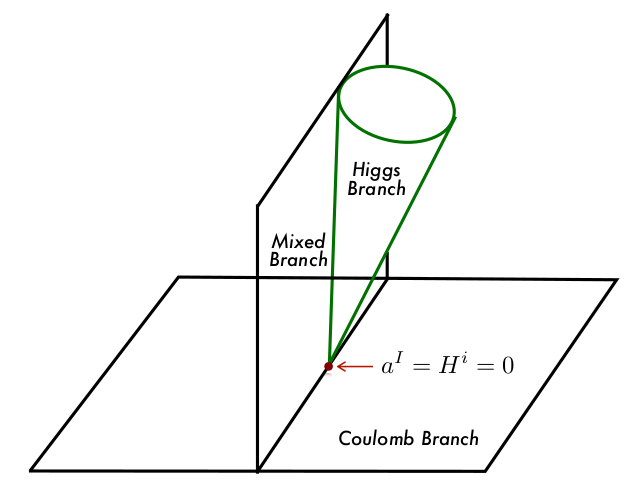
\includegraphics[scale=0.35]{Pictures/classicalmodulispace.png}
            \caption{$\mN=2$ classical moduli space, from \cite{bertolinisusy}.}
        \end{figure}

        \begin{examp}
            Taking $G=\SU(N)$, the Weyl group is $S_{N-1}$ and the rank is $N-1$. A natural set of $\U(1)^{N-1}\times S_{N-1}$ invariant coordinates on the $(N-1)$-dimensional moduli space is $\M_c=\C^{N-1}/S_{N-1}$ can be shown to be
            \begin{equation}
                u_2=\sum_{i<j}a^ia^j,\quad u_3=\sum_{i<j<k}a^ia^ja^k,\quad \dots,\quad u_N=a^1\dots a^N, \qquad i,j,k=1,\dots,N
            \end{equation}
            where $\phi=\text{diag}(a^1,\dots,a^N)$ with $\sum^N_{i=1} a^i=0$.
        \end{examp}

    \subsection{Quantum moduli space of vacua}

        We have seen the classical part of the story for the moduli space. How does quantum corrections change it? This a complicated question and it the goal of these notes to explain how to answer it. At this point, we can already anticipate three very important properties of the quantum moduli space $\M_q$:
        \begin{enumerate}
            \item \textbf{Product structure:} the $\mN=2$ selection rule that dictates that the classical moduli space has to look locally like a product \eqref{eq:classicalmodulispaceproduct} comes from the supersymmetry algebra and therefore also holds at the quantum level. Hence, locally, we have
            \begin{equation}
                \M_q = \M^V_{q}\times\M^H_{q}.\label{eq:quantummodulispaceproduct}
            \end{equation}
            \item \textbf{The Higgs branch:} $\mN=2$ supersymmetry implies that the special Kähler metric on $\M^V_{c}$ and that the imaginary part if the generalized complexified gauge coupling $\tau_{IJ}$ are related. The former only depends on the scalar fields $\phi^I$ while the latter undergoes renormalization at one-loop. Its quantum-corrected expression is a function of the strong-coupling scale $\Lambda$, which therefore appears in the lagrangian in the same way as a VEV of a scalar belonging to a vector multiplet. However, the metric does not depend on those scalars and therefore does not depend on $\Lambda$ either. This means that taking the limit $\Lambda\to0$ will not change the metric. In other words, the Higgs branch is classically exact:
            \begin{equation}
                \M^H_{c}=\M^H_{q}.
            \end{equation}
            On the other hand, the metric on the Coulomb brach can receive quantum corrections and solving the theory boils down to finding this metric. This explain why we will mostly focus on the Coulomb branch metric.
            \item \textbf{Existence of moduli space:} in $\mN=2$ theories, the moduli space can never be completely lifted, unlike for $\mN=1$ theories for example. This is obvious for the Higgs branch; since it is classicaly exact, existance at classical level implies existence at the quantum level. For the Coulomb branch on the other hand, it is less obvious and it is explained in \cite[p. 282]{bertolinisusy}.
        \end{enumerate}

        What about singularities? The classical moduli space admits singularities of enhanced gauge symmetry. However, the quantum moduli space cannot admit such singularities. This a result that we will show in the following. More precisely, it can have singularities where some massive particles become massless but those particles will never be gauge fields. There are no point of enhanced gauge symmetry and the theory is always in the Coulomb phase. In stead, there exist other types of singularities, such as Argyres-Douglas singularities for example, where mutually non-local particles become simultaneously massless.

        \begin{figure}[H]
            \centering
            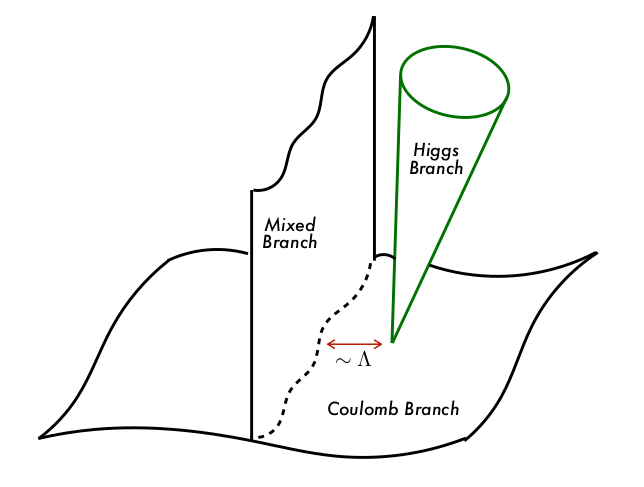
\includegraphics[scale=0.35]{Pictures/quantummodulispace.png}
            \caption{$\mN=2$ quantum moduli space, from \cite{bertolinisusy}.}
        \end{figure}

\section{Monopoles, dyons and electric-magnetic duality}

    Let us start by considering electromagnetism without matter, i.e. a non-supersymmetric pure gauge theory with gauge group $\U(1)$. The action is given by
    \begin{equation}
        S[A]=\frac{1}{4g^2}\int F\wedge\star F
    \end{equation}
    with $F=\d A$ and the equations of motion are
    \begin{equation}
        \d\star F=0,\qquad \d F=0.
    \end{equation}
    They are invariant under the transformation
    \begin{equation}
        S:F\mapsto\star F,\star F\mapsto-F
    \end{equation}
    which exchanges the electric and magnetic fields. It is called \emph{S-duality}. In the presence of electric sources, the theory can still be invariant under S-duality if one adds magnetic sources, i.e. \emph{monopoles}. The action reads
    \begin{equation}
        S[A]=\frac{1}{4g^2}\int F\wedge\star F+A\wedge j_e-A\wedge j_m
    \end{equation}
    \todo{verify expression f the action}and the equations of motion are now Maxwell equations:
    \begin{equation}
        \d\star F=j_e,\qquad \d F=-j_m.
    \end{equation}
    S-duality now acts as
    \begin{equation}
        S:F\mapsto\star F,\qquad \star F\mapsto-F,\qquad j_e\mapsto j_m,\qquad j_m\mapsto-j_e.
    \end{equation}
    The presence of magnetic monopoles implies quantization of the charges: a theory with electric charge $q$ and magnetic charge $p$ can only be consistently quantized if the \emph{Dirac quantization condition}
    \begin{equation}
        qp=2\pi n,\qquad n\in\Z
    \end{equation}
    holds The magnetic and electric charges are therefore inversely proportional, if one is big, the other must be small. Therefore, S-duality is a strong-weak duality coupling duality. It not a symmetry of the theory since it acts on the couplings. Rather, it map s a description of the theory to another description of the same theory.

    One can always add the term
    \begin{equation}
        \frac{\theta e^2}{32\pi^2}\tr(F\wedge\star\tilde{F}),
    \end{equation}
    called the $\theta$-term and it does not change Maxwell equation. In the presence of a magnetic monopole, a $\theta$-terms has an interesting physical effect, called the \emph{Witten effect}: a particle with magnetic charge $p=\frac{4\pi}{e}$ and $\U(1)$ electric charge $n_ee$ has the following electric charge:
    \begin{equation}
        q = n_ee-\frac{\theta e^2}{8\pi^2}p=n_ee-\frac{\theta e}{2\pi}.
    \end{equation}
    Therefore the magnetic charge contributes to the electric charge. In particular, a magnetic monopole always carries an electric charge.

    States that are both magnetically and electrically charged are called \emph{dyons}. In the presence of such states, the Dirac quantization condition is generalized to the \emph{Dirac-Schwinger-Zwanziger} quantization condition:
    \begin{equation}
        q_1p_1-q_2p_2=2\pi n,\qquad n\in\Z.
    \end{equation}



\section{Low energy effective actions}

    \subsection{General discussion}

        The leading dynamic of any (supersymmetric or non-supersymmetric) asyptotically free theory around a vacua where the potential vanishes is governed by massless fields. In this limit, the theory is scale invariant, by definition, and is at an IR fixed point of the RG flow. However, the nature of this IR fixed point can be if two kinds:
        \begin{itemize}
            \item If no massless fields are present initially, there are no propagating degrees of freedom in the low-energy limit and the IR fiwed point is trivial.
            \item If the initial theory contains some massless fields, the theory can be in a free or interacting phase and the IR fixed point is non-trivial.
        \end{itemize}
        
        \begin{theorem}[Colemann-Gross]
            In four spacetime dimensions, any theory of scalars, spinors and abelian gauge fields flows in the IR to a free (or trivial if everything gets a mass) theory.
        \end{theorem}
        This provides us with a necessary condition for having an interacting conformal field theory at low energy: there must be at least one massless non-abelian gauge field in the low-energy effective action. Note there are no general tool to study strongly coupled, interacting conformal field theories.

        Motivated by the previous discussion, we will only focus on effective theories that have scalars, spinors and abelian gauge fields. This is not such a restriction since for both $\mN=2$ and $\mN=4$ theories, a large fraction of the moduli space enjoys such an abelian, IR-free phase.
        
        What is the field content of the effective action ? A massless charged field will becomes massive though Higgs mechanism and then decouple as the energy scale is taken to be lower than the mass, so it cannot appear in the effective action. If, on the contrary, a massless is charged, it would still decouple and not appear in the effective action. We conclude that only massless neutral fields can appear in the low energy effective action. The low energy effective lagrangian must be of the form
        \begin{equation}
            \L = g_{ij}(\phi)\p\mu\phi^i\p^\mu\phi^j+\frac{1}{2}\Im[\tau_{IJ}(\phi)\F^I_{\mu\nu}\F^{J~\mu\nu}]+\text{ fermions}
        \end{equation}
        where $i,j$ run on neutral massless scalar fields and $I,J$ on abelian gauge fields. The \emph{complexified gauge coupling} $\tau_{IJ}$ and the field strength are defined as follows:
        \begin{equation}
            \tau_{IJ}=\frac{\theta_{IJ}}{2\pi}+\frac{4\pi i}{g^2_{IJ}}.
        \end{equation}
        The sigma-model metric $g_{ij}(\phi)$ is the metric on the moduli space $\M$, whose coordinates are the massless scalar fields VEV's.

    \subsection{$\mN=2$ effective action}

        Let us focus on $\mN=2$ supersymmetric theories and start from the most general asymptotically free renormalizable action. This action is fully characterized by the gauge group $G$ and the matter content, it is given by \eqref{eq:N2lag} for a pure gauge theory.

        It is known (just from supersymmetry) that the low energy effective lagrangian\footnote{By ``low energy effective lagrangian'', we mean the part of the effective lagrangian that contains the leading terms when the momenta vanish. In the full effective lagrangian there are of course infinitely many higher derivative terms. These are not governed by holomorphic quantities and we therefore have no control on them regarding quantum corrections.} must be of the for the form
        \begin{equation}
            \L^{\mN=2}_{\text{eff}} = \frac{1}{4\pi}\Im\left[\int\d^2\theta\d^2\bar{\theta}~K(\Phi,\bar{\Phi})+\int\d^2\theta\left(\frac{1}{2}\sum\tau(\Phi)W^\alpha W_\alpha\right)\right]
        \end{equation}
        with
        \begin{equation}
            K(\Phi,\bar{\Phi})=-\frac{i}{32\pi}\pdv{\F(\Phi)}{\Phi^a}\bar{\Phi}^a+\text{h.c.},\qquad \F_{ab}(\Phi)=\pdv{\F(\Phi)}{\Phi^a}{\Phi^b}.\label{eq:effectivelagftcs}
        \end{equation}
        It is therefore completely determined by the holomorphic function $\F$, called the \emph{prepotential}. The same model can be obtained from the usual lagrangian by just relaxing the renormalizability condition. We recover a renomalizable lagrangian by taking $\F(\Phi)=\frac{1}{2}\tau\tr\Phi^2$

        The map $K(A,\bar{A})$ is the Kähler potential, which gives a supersymmetric non-linear sigma-model for the field $\Phi$. It defines a metric on the moduli space as
        \begin{equation}
            ds^2=g_{i\bar{j}}(\Phi,\bar{\Phi})\d\Phi^a\d\bar{\Phi}^b = \pdv{K(\Phi,\bar{\Phi})}{\Phi^a}{\bar{\Phi}^b}\d\Phi^a\d\bar{\Phi}^b.
        \end{equation}
        From \eqref{eq:effectivelagftcs}, we see that 
        \begin{equation}
            ds^2=\pdv{K(\Phi,\bar{\Phi})}{\Phi^a}{\bar{\Phi}^b}\d\Phi^a\d\bar{\Phi}^b = \Im\left[\pdv{\F(\Phi)}{\Phi^a}{\Phi^b}\right]\d\Phi^a\d\bar{\Phi}^b
        \end{equation}
        thus the coefficients $\F_{ab}$ can be interpreted as coupling constant but they are also related to the metric on the moduli space.

        The potential is the effective lagrangian is given by
        \begin{equation}
            V(\phi,\phi^\dagger)=-\frac{1}{2\pi}\left(\Im\F_{ab}(\phi)\right)^{-1}[\phi^\dagger,\F_c(\phi)T_c]^a[\phi^\dagger,\F_d(\phi)T_d]^b.
        \end{equation}
        The Coulomb branch is therefore a Kähler manifold. Since the the Kähler potential can be written in terms of a holomorphic function as in \eqref{eq:effectivelagftcs}, it is more precisely a special Kähler manifold.

        If we were to add a hypermultiplet, we would have to additional complex scalars (one from each chiral superfields of the decomposition of the hypermultiplet). This new sigma-model would then define quaternionic manifold known as a Hyperkähler manifold. Due to the existence of those two sets of scalars (those belonging to the vector multiplet and those belonging to the hypermultiplet), the classical moduli space has the more general form
        \begin{equation}
            \M_c=\M^V\times\M^H
        \end{equation}
        where $\M^V$ is a Kähler manifold and $\M^H$ a Hyperkähler manifold.


\section{$\SU(2)$ $\mN=2$ supersymmetric Yang-Mills theory}

\section{Generalization to other groups}

\section{SW geometry from string duality}

\appendix

\section{Weyl group}

    \subsection{Root systems}

        Let $V$ be a finite-dimensional vector space with inner product $\prod{\cdot}{\cdot}$. A \emph{root system} $\Phi$ in $V$ is a finite set of non-zero vectors, called \emph{roots}, that satisfy the following conditions:
        \begin{enumerate}
            \item $\text{span}\Phi=V$,
            \item if $\alpha\in\Phi$, the only scalar multiples of $\alpha$ in that belongs to $\Phi$ are $\alpha$ itself and $-\alpha$,
            \item for all $\alpha\in\Phi$, the set $\Phi$ is closed under reflection through the hyperplane orthogonal to $\alpha$. In other words, $\Phi$ it is closed under the maps
            \begin{equation}
                s_\alpha(\beta)\equiv\beta-2\frac{\prod{\alpha}{\beta}}{\prod{\alpha}{\alpha}}\alpha,
            \end{equation}
            \item integrability: if $\alpha,\beta\in\Phi$, the projection of $\beta$ onto the line through $\alpha$ is an integer or half-integer multiple of $\alpha$, i.e.
            \begin{equation}
                (\alpha,\beta)\equiv 2\frac{\prod{\alpha}{\beta}}{\prod{\alpha}{\alpha}}\in\N.
            \end{equation}
        \end{enumerate}
        Two root systems $(V_1,\Phi_1)$ and $(V_2,\Phi_2)$ are \emph{isomorphic} if there is an invertible linear transformation $V_1\to V_2$ which sends $\Phi_1$ to $\Phi_2$ such that foreach pair of roots, the number $(\alpha,\beta)$ is preserved. The \emph{root lattice} of a root system $\Phi$ is the $\Z$-submodule of $V$ generated by $\Phi$.

        Given a root system $\Phi$, we can always choose (in many ways) a set of \emph{positive roots}. This is a subset $\Phi^+$ of $\Phi$ such that
        \begin{itemize}
            \item for each root $\alpha\in\Phi$, exactly one the the roots $\alpha,-\alpha$ belongs to $\Phi^+$
            \item for any two distinct $\alpha,\beta\in\Phi^+$ such that $\alpha,\beta$ is a root, $\alpha+\beta\in\Phi^+$
        \end{itemize}
        For a chosen set of positive roots, elements of $-\Phi^+$ are called \emph{negative roots}. A set of positive root can be constructed by choosing a hyperplane not containing any root and setting $\Phi^+$ to be all the roots lying on a fixed side of this hyperplane. Actually, all sets of positive roots arises in this way.

        An element of $\Phi^+$ is called a \emph{simple root} (or \emph{fundamental root}) if it cannot be written as the sum of two elements of $\Phi^+$. The set $\Delta$ of simple roots is referred to as a \emph{base} of $\Phi^+$, and it is a basis of the vector space $V$ with the following additional properties:
        \begin{itemize}
            \item every root $\alpha\in\Phi$ is a linear combination of elements of $\Delta$ with integer coefficients,
            \item for each $\alpha\in\Phi$, the coefficients in the previous point are either all non-negative or all non-positive.
        \end{itemize}
        For each root system $\Phi$, there are many different choices of sets of positive roots and of simple roots, but any two sets of positive roots differ by the action of the Weyl group, that will be defined next.

    \subsection{Weyl group}

        The \emph{Weyl group} $W$ of a root system $\Phi$ is the group generated by all the maps $s_\alpha$ where the product is the composition of maps. $W$ is a then a subgroup of the orthogonal group $\O(V)$ and, since the maps $s_\alpha$ and that they leave $\Phi$ invariant and that $\Phi$ is finite, $W$ is necessarily a finite group.

        \begin{examp}
            Let us work out the example of the root system $A_2$ in details, the root system of the Lie algebra $\mathfrak{su(3)}$. After computing the fundamental roots of the Lie algebra, we find that
            \begin{equation}
                V=\{v\in\R^3|\sum_i v_i=0\}
            \end{equation}
            and that the roots are given by
            \begin{equation}
                \alpha_{12}=e_1-e_2,\qquad
                \alpha_{23}=e_2-e_3,\qquad
                \alpha_{31}=e_3-e_1
            \end{equation}
            and their opposite, where $\{e_i\}_{i=1,\dots,3}$ is the canonical basis of $\R^3$. One can show that the group generated by the maps $s_{\alpha_{ij}}$ is $W=S_3$.
        \end{examp}

        More generally, the Weyl group for $A_n$ is $S_{n+1}$.

    \subsection{Dynkin diagrams}

        A root system is \emph{irreducible} if it cannot be partitioned into the union of two proper subsets $\Phi=\Phi_1\cup\Phi_2$, such that $\prod{\alpha}{\beta}=0$ for all $\alpha\in\Phi_1$ and $\beta\in\Phi_1$. Irreducible root systems correspond to a certain graph, the \emph{Dynkin diagram}. Given a root system and a set of simple roots $\Delta$, the vertices of the associated Dynkin diagram correpsond to the roots in $\Delta$ and edges are drawn between the vertices suing the following rules:
        \begin{itemize}
            \item no edge if the vectors are orthogonal,
            \item an undirected single edge if they make and angle of $120$ degrees,
            \item a directed double edge if they make an angle of $135$ degrees,
            \item a directed triple edge if they make an angle of $150$ degrees.
        \end{itemize}
        The directed edges point towards the shorter vector. 
        
        Although there are many choices for the set of simple roots, the Weyl group acts transitively on them. Consequently, the Dynkin diagram is independent of this choice. Actually, there is a one-to-one correspondence between root systems and Dynkin diagrams. The classification of these graphs is a simple matter of combinatorics, and induces a classification of irreducible root systems.

    \subsection{Semisimple Lie algebras and roots}

        Let $\g$ be a finite-dimensional semisimple Lie algebra over an algebraically closed field of characteristic $0$. The structure of $\g$ can be described by a certain subalgebra in it. This subalgebra is the \emph{Cartan subalagebra} (CSA), it is defined as the maximal abelian subalgebra of $\g$ and we denote by $\h$. Consequently, since $\ad([x_1,x_2])=[\ad(x_1),\ad(x_1)]$ for all $x_1,x_2\in\g$, by definition of a representation of a Lie algebra, all the operators $\ad(h)$ for $h\in\h$ commute. So the CSA is precisely the maximal subalgebra of $\g$ such that the operators $\ad(h)$ are simultaneously diagonalizable. For each linear functional $\alpha\in\h^*$, we define
        \begin{equation}
            \g_\alpha\equiv \{x\in\g|[h,x]=\alpha(h)x\text{ for all }h\in\h\}.
        \end{equation}
        The primordial result linking roots and Lie algebras is the \emph{root space decomposition}: given a CSA $\h$, it holds that $\g_0=\h$ and there is a decomposition
        \begin{equation}
            \g=\h\oplus\bigoplus_{\alpha\in\Phi}\g_\alpha
        \end{equation}
        where $\Phi$ is the set of all non-zero linear functionals $\alpha$ of $\h$ such that $\g_\alpha\neq\{0\}$. Moreover, for each $\alpha,\beta\in\Phi$,
        \begin{itemize}
            \item $[\g_\alpha,\g_\beta]\subseteq\g_{\alpha+\beta}$ with equality if $\alpha+\beta\neq0$,
            \item $[\g_\alpha,\g_{-\alpha}]\oplus\g_\alpha\oplus\g_{-\alpha}\cong\mathfrak{sl}_2$ as a Lie algebra,
            \item $\dim\g_\alpha=1$ and $\dim\g=\dim\h+\#\Phi$,
            \item with respect to the Killing form $B$, $\g_\alpha$ and $\g_\beta$ are orthogonal to each other if $\alpha+\beta\neq0$, the restriction of $B$ to $\h$ is non-degenerate,
            \item $\Phi$ is a root system.
        \end{itemize}
        
        Let us take $\h_\alpha\in\h$, $e_\alpha\in\g_\alpha$ and $f_\alpha\in\g_{-\alpha}$ with the commutation relations
        \begin{equation}
            [e_\alpha,f_\alpha]=h_\alpha,\qquad [h_\alpha,e_\alpha]=2e_\alpha,\qquad [h_\alpha,f_\alpha]=-2f_\alpha,
        \end{equation}
        i.e. $h_\alpha,e_\alpha,f_\alpha$ is the standard basis of $\mathfrak{sl}_2$. Let us take $\Delta=\{\alpha_1,\dots,\alpha_l\}$ a set of simple roots of $\Phi$, with $\alpha_i\in\h^*$ and denote $e_i\equiv e_{\alpha_i}$, etc. Then, the $3l$ generators $e_i,f_i,h_i$ generate $\g$. They are called the \emph{Chevalley generators}. They satisfy the \emph{Serre relations}
        \begin{align}
            &[h_i,h_j] = 0,\\
            &[e_i,f_i] = h_i,\quad [e_i,f_j]=0, i\neq j,\\
            &[h_i,e_j] = a_{ij}e_j,\quad [h_i,f_j]=-a_{ij}f_j,\\
            &\ad(e_i)^{-a_{ij}+1}(e_j) = \ad(f_i)^{-a_{ij}+1}(j_j)=0,i\neq j,
        \end{align}
        with $a_{ij}\equiv\alpha_i(h_j)$.

        In this language, the Weyl group it the group of linear transformations of $\h^*\cong\h$ generated by the $s_\alpha$'s that can be written as acting on $\h^*$ as $s_\alpha:\h^*\to\h^*:\gamma\mapsto\gamma(h_\alpha)\alpha$. It is an important symmetry of the problem. For example, the weights of any finite-dimensional representation of are invariant under the Weyl group.

    \subsection{Weights}

        Let $V$ be a representation of $\g$ over $\C$, $\g$ being semisimple Lie algebra with CSA $\h$. For a given $\lambda\in\h^*$, the \emph{weight space} of $V$ with weight $\lambda$ is the subspace $V_\lambda$ given by
        \begin{equation}
            V_\lambda\equiv \{v\in V| h\cdot v =\lambda(h)v\text{ for all }h\in\h\}.
        \end{equation}
        The \emph{weight} of a representation $V$ is a linear functional such that the correspondinf weight space is non-zero. Non-zero vectors of the weight space are called \emph{weight vectors}, they are a simultaneous eigenvector for the action of all the elements of $\h$, with eigenvalue given by $\lambda$. 

\printbibliography

\end{document}